\documentclass[qualitaetssicherung.tex]{subfiles}

\begin{document}

\section{Chrome - Darstellungs von Settings}
	\subsection{Einleitung}
	Um zu wissen, wie schnell wir die Settings darstellen können und mit wieviel Aufwand die Darstellung verbunden ist, können wir einfach versuchen ziemlich schnell auf verschiedene GUI-Elemente zu klicken und beobachten, wie lange es dauert, bis alles neu gezeichnet wird. Selbstverständlich klicken wir (hoffentlich) langsamer, als unser Rechner die klicks verarbeitet. Um alles zumindest teilweise zu automatisieren (eine vollständige Automatisierung ist auch möglich, in diesem Fall macht aber wenig Sinn), verwenden wir das Programm Autohotkey. Autohotkey kann verschiedene Skripte öffnen, die Mausbewegungen, Klicks, Tastatureingaben... usw. beschreiben.
	\subsection{Ablauf}
	\begin{itemize}
	\item Wir schreiben ein Skript und stellen es ein, dass wir alle 30 Millisekunden einmal klicken wollen.
	\item Wir öffnen Chrome und stellen sicher, dass Settings angezeigt wird (Abb. ~\ref{settings_speedtest}).
	\item Wir lassen das Skript laufen und beobachten, was passiert.
	\item Wenn wir mit dem Cursor die numerische Eingaben (HTML Input/number) verändern, deren Darstellung tief in Chrome verankert ist und wir annehmen können, dass es so schnell wie möglich (oder sinnvoll) erfolgt, stellen wir fest, dass Chrome auf Windows etwa 10 Klicks pro Sekunde verarbeitet und es nicht an der CPU-Auslastung liegt. Wir haben versucht 33-mal pro Sekunde zu klicken. Was bedeutet dies für uns? Wenn wir 10 fps erreichen ohne dabei den Prozessor erheblich zu belasten, dann sind wir erfolgreich.
	\item Hinweis: Eine Videoaufnahme vom Benchmark ist vorhanden.
	\item Wie wir auf dem Video auch sehen können, erreichen wir 10 fps und verursachen dabei 16\% CPU-Auslastung. Wir haben drei Kerne, die alle mit einer Geschwindigkeit von 2.4 GHz laufen.
	\item Fazit: Das Ergebnis wäre bei einem Programm, das nativ ausgeführt wird und in C geschrieben ist als schlecht zu beurteilen, in unserem Fall aber nicht, wir haben die Ziele erreicht, die Geschwindigkeit, die wir erreicht haben genügt.
	
	\begin{figure}[H]
    \textbf{Settings geöffnet in Chrome}\par\medskip
    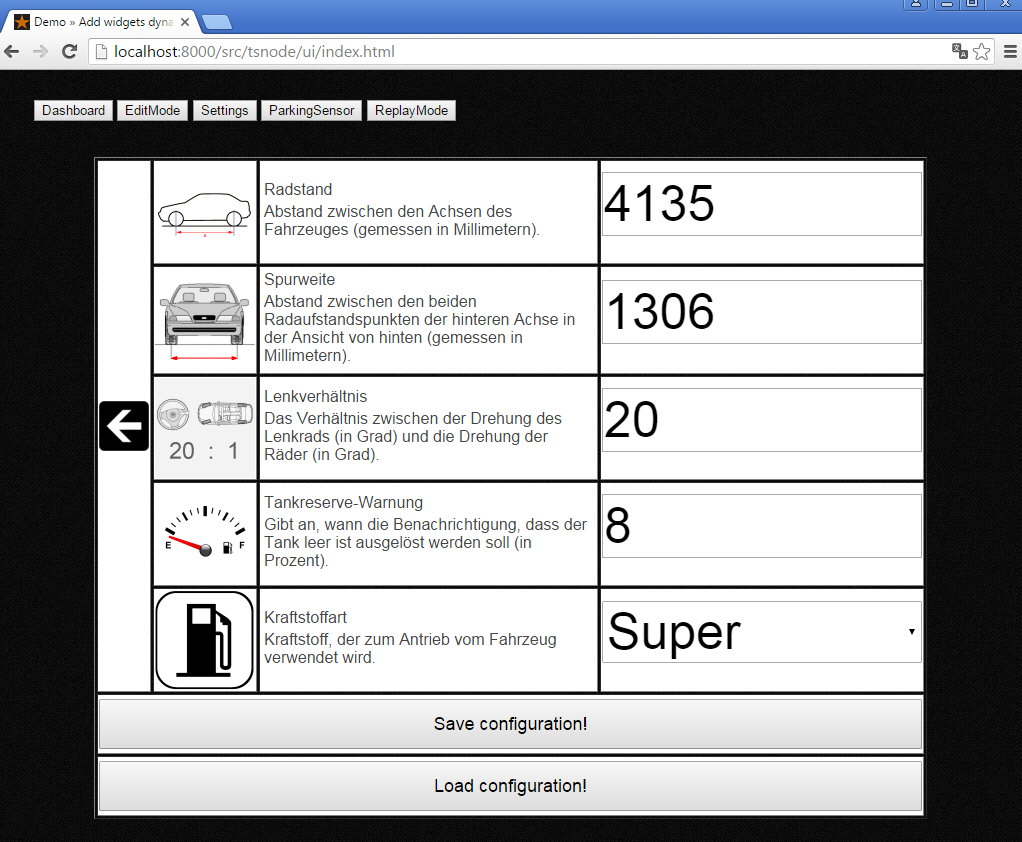
\includegraphics[width=0.99\textwidth]{Images/settings-speedtest.png}
    \caption{Durchschnittliche Auslastung eines CPU-Kerns: 50\%}
		\label{settings_speedtest}
	\end{figure}
	\end{itemize}
	
\end{document}